\chapter{Results}
The algorithm developed within this thesis was evaluated on ten DCE-MRI sequences of ten different participants. For each of the participant one of the two  DCE-MRI sequences was chosen randomly.

The segmentation of the pelvis was evaluated with \textit{Dice similarity coefficient} (\textit{DC}) given by the formula \cite{dice1945measures}:
\begin{equation}
	\label{eq:dice}
	DC = \dfrac{2|A\cap{}B|}{|A|+|B|},
\end{equation}
where |A| and |B| are the number of voxels in pelvis detected  in the automatic segmentation routine and the number of voxels in ground truth labelled organoleptically, respectively, whereas $|A\cap{}B|$ is the number of common voxels.
The average accuracy of the pelvis segmentation was equal to DC~=~0.86\,$\pm$\,0.06.

The SKGFR values of the left and right kidney, as well as total GFR for each of the participants obtained in the examination of the MRI sequences applying different PK models are shown in Table~\ref{tab:results}. Also, the GFR values obtained with chemical methods were included in the table for comparison. \textit{Measured GFR} (mGFR) is a value obtained in iohexol-GFR test, whereas \textit{estimated GFR} (eGFR) is the one derived from the SCr blood test.

For each of the method (different PK models and SCr blood test) its degree of agreement with the reference method  (iohexol-GFR test) was assessed. For this purpose the Bland–Altman plots \cite{bland1986statistical} were drawn as shown in Figure \ref{fig:baltman}. 
This type of plot is a scatter one, in which the difference between the measurement of the examined method and the reference method is plotted against the average of these measurements.
The plot indicates the central tendency (bias) as the robust grey line calculated as the mean difference of the measurements. The so-called \textit{limits of agreement} (LoA) are denoted as grey dashed lines and indicate the interval, within which 95\% of the measurements is expected to lay.

\begin{landscape}
\begin{table}[H]
\centering
\caption{GFR values derived from DCE-MRI using different PK models and values obtained with chemical methods}
\label{tab:results}
\begin{threeparttable}
\rowcolors{3}{}{middleblue!30}
\renewcommand{\arraystretch}{1.5}
\begin{tabular}{l r r c R{0.64cm} R{0.64cm} >{\columncolor{magenta!35}}R{0.64cm} c R{0.64cm} R{0.64cm} >{\columncolor{magenta!35}}R{0.64cm} c R{0.64cm} R{0.64cm} >{\columncolor{magenta!35}}R{0.64cm} c R{0.64cm} R{0.64cm} >{\columncolor{magenta!35}}R{0.64cm}}
	\toprule
	%\multirow{3}{*}{\shortstack[l]{\textbf{Subject}\\ \textbf{no.}}}&
	\multirow{3}{*}{\textbf{No.}}&
	\multirow{3}{*}{\textbf{mGFR}}&
	\multirow{3}{*}{\textbf{eGFR}}& \phantom{abc}&
	\multicolumn{15}{c}{\textbf{MRI GFR}}\\ \cmidrule{5-19}
	&&&& \multicolumn{3}{c}{\textbf{TK}} & \phantom{abc}&
    \multicolumn{3}{c}{\textbf{ETK}} & \phantom{abc}&
    \multicolumn{3}{c}{\textbf{PR}} & \phantom{abc}&
    \multicolumn{3}{c}{\textbf{2CXM}}\\
    \cmidrule{5-7} \cmidrule{9-11} \cmidrule{13-15} \cmidrule{17-19}
   \rowcolor{white} &&&& \textbf{L} & \textbf{R} & \cellcolor{white} \textbf{T} & & \textbf{L} & \textbf{R} & \cellcolor{white} \textbf{T} && \textbf{L} & \textbf{R} & \cellcolor{white} \textbf{T} && \textbf{L} & \textbf{R} & \cellcolor{white} \textbf{T}\\ 
    \toprule
    %\rowcolors{2}{}{beaublue!50}
  	1  & 97  & 126 & & 85 & 82 & 167 & & 66 & 61 & 127 & & 25 & 23 & 48 && 42 & 31 & 72 \\
  	2  & 100 & 111 & & 75 & 62 & 137 & & 61 & 53 & 115 & & 21 & 20 & 41 && 61 & 50 & 111 \\
  	3  & 104 & 125 & & 48 & 62 & 111 & & 42 & 53 & 95  & & 18 & 22 & 40 && 39 & 44 & 83 \\
  	4  & 101 & 116 & & 55 & 49 & 105 & & 47 & 42 & 89  & & 14 & 12 & 26 && 61 & 53 & 114    \\
  	5  & 90  & 80  & & 71 & 76 & 146 & & 61 & 62 & 123 & & 17 & 17 & 34 && 38 & 34 & 72 \\
  	6  & 89  & 93  & & 42 & 48 & 90  & & 34 & 40 & 74  & & 12 & 15 & 27 && 42 & 37 & 79 \\
  	7  & 102 & 114 & & 48 & 52 & 100 & & 36 & 39 & 75  & & 11 & 13 & 25 && 51 & 51 & 101 \\
  	8  & 103 & 123 & & 50 & 61 & 111 & & 38 & 47 & 85  & & 12 & 13 & 25 && 48 & 51 & 99 \\
  	9  & 87  & 100 & & 44 & 64 & 108 & & 35 & 57 & 92  & & 18 & 25 & 42 && 52 & 37 & 89 \\
  	10 & 97  & 115 & & 59 & 64 & 123 & & 46 & 50 & 96  & & 17 & 18 & 35 && 52 & 47 & 100 \\

  \bottomrule

\end{tabular}
\begin{tablenotes}%
\footnotesize{}%
\item L and R are SKGFR for left and right kidneys, respectively, whereas T is the total GFR.
\item TK, ETK, PR, 2CXM are particular PK models. 
\item Note that $L+R = T$ is not always satisfied because of the rounding error.
\item All GFR values are expressed in mL/min$^{-1}$/1.73\,m$^2$.
    \end{tablenotes}
	\end{threeparttable}
\end{table}
\end{landscape}


\begin{figure}[H]
%\captionsetup[subfigure]{labelformat=empty,textformat=simple}
	\centering
	\sidesubfloat[]{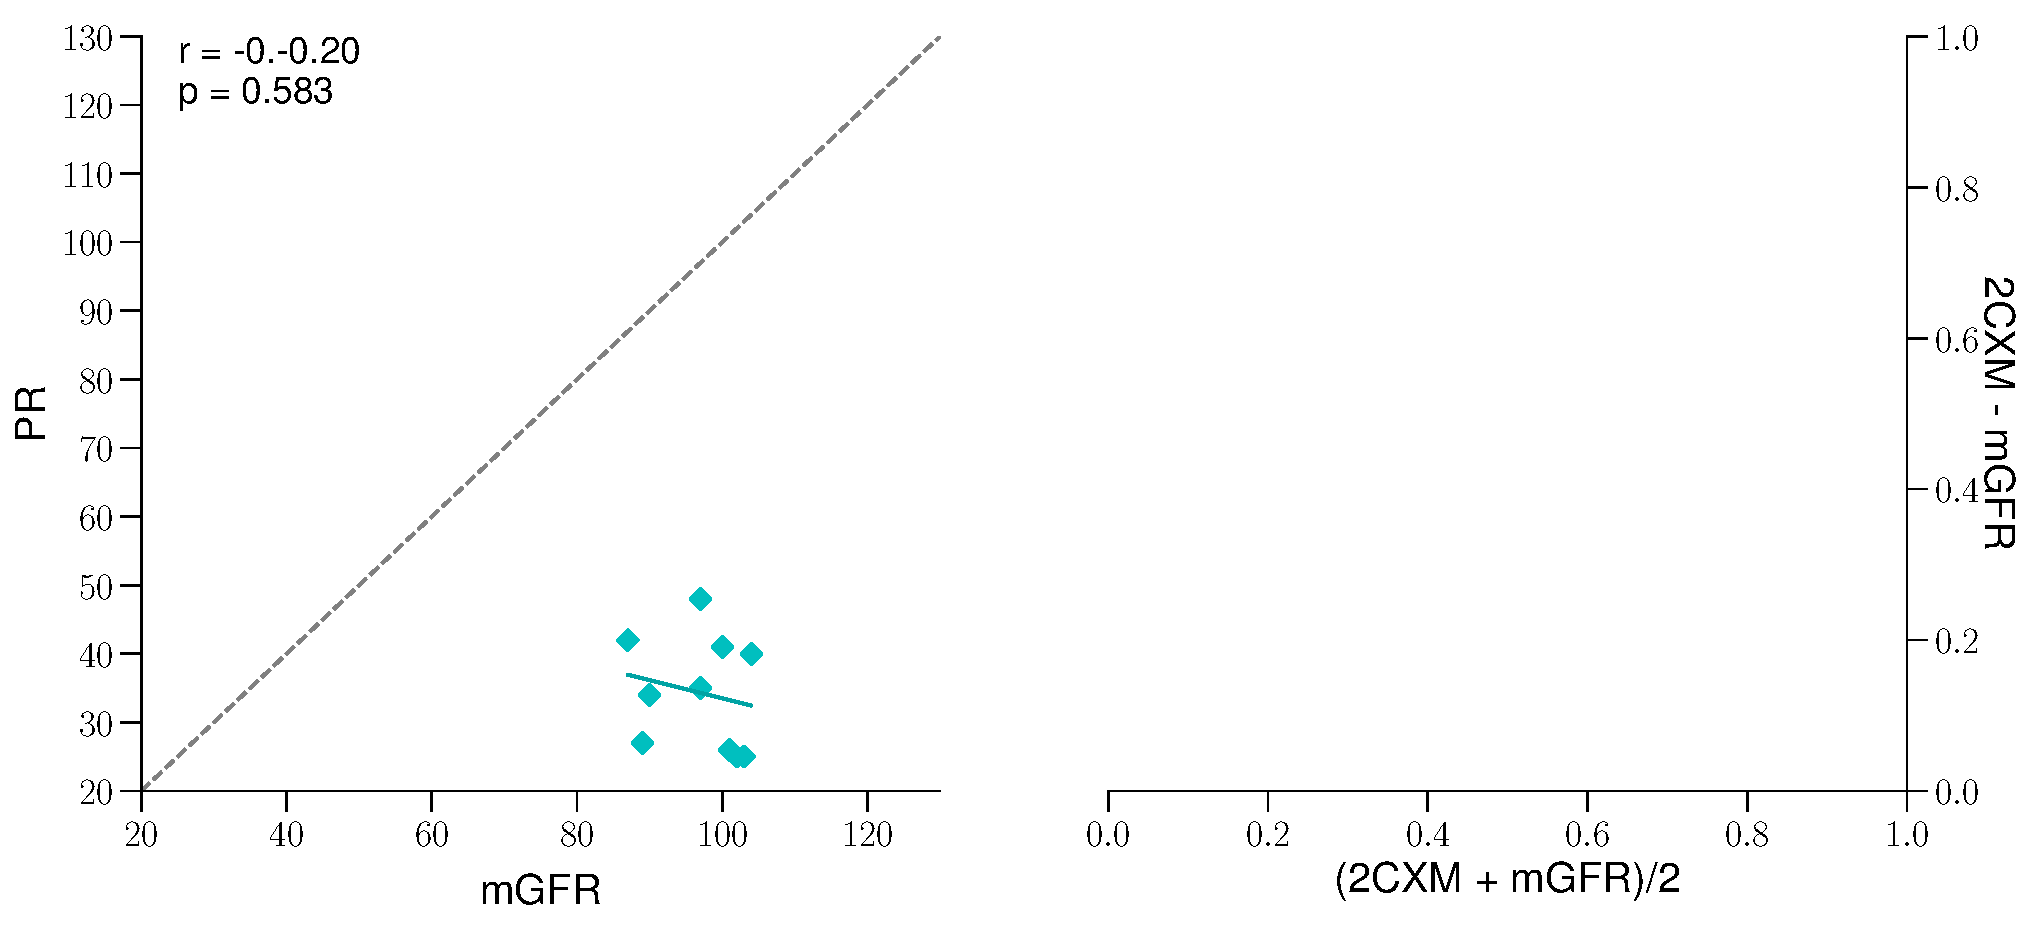
\includegraphics[width=0.42\linewidth]{baltman-egfr}} \\ \vspace{10pt}  
 	\sidesubfloat[]{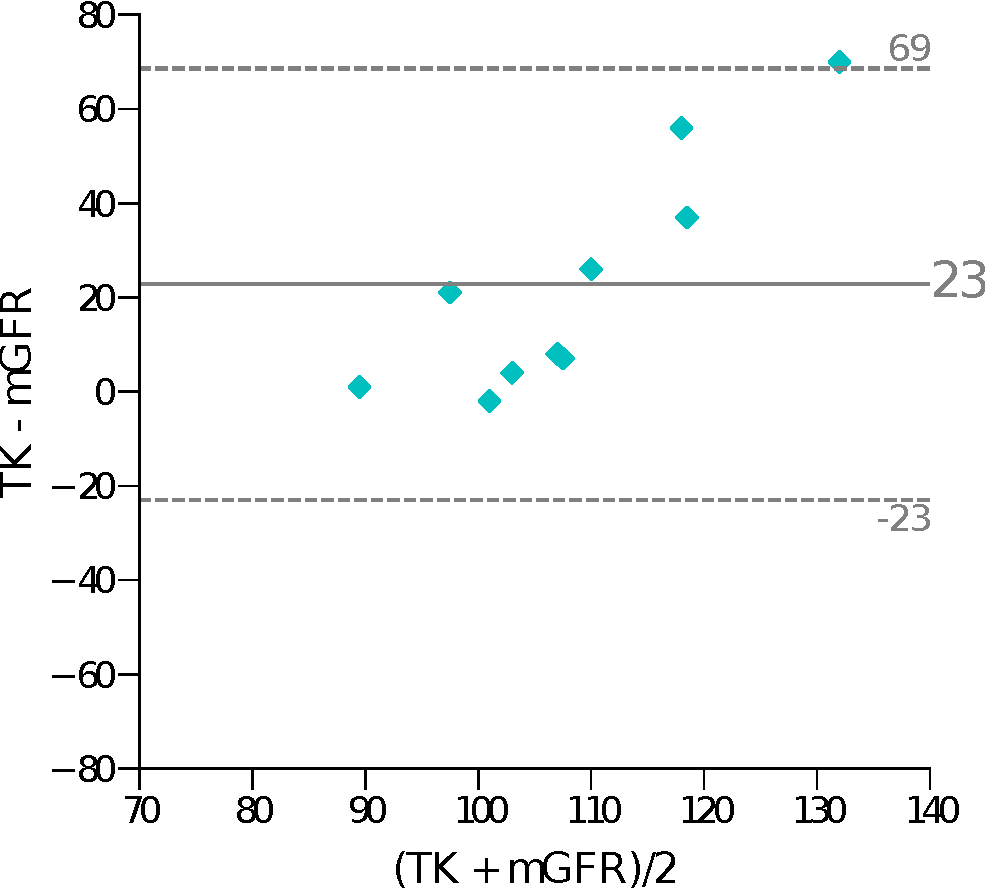
\includegraphics[width=0.42\linewidth]{baltman-tk}} \hfill \sidesubfloat[]{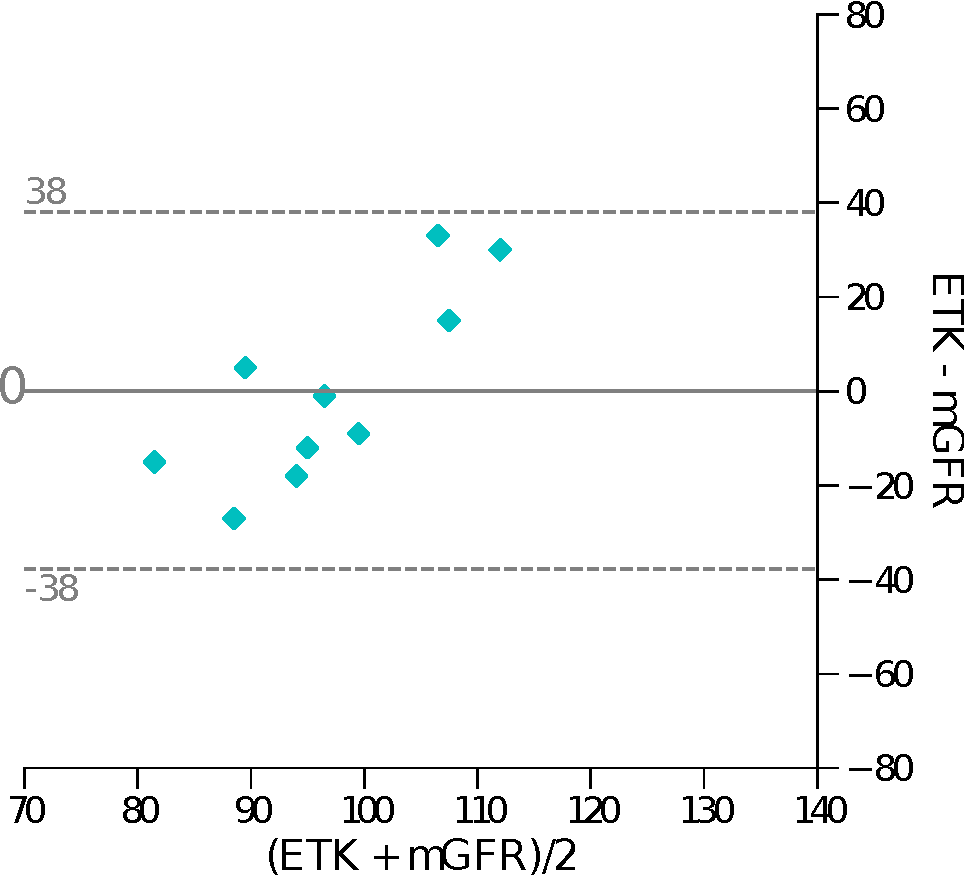
\includegraphics[width=0.42\linewidth]{baltman-etk}} \\ \vspace{10pt}   
	\sidesubfloat[]{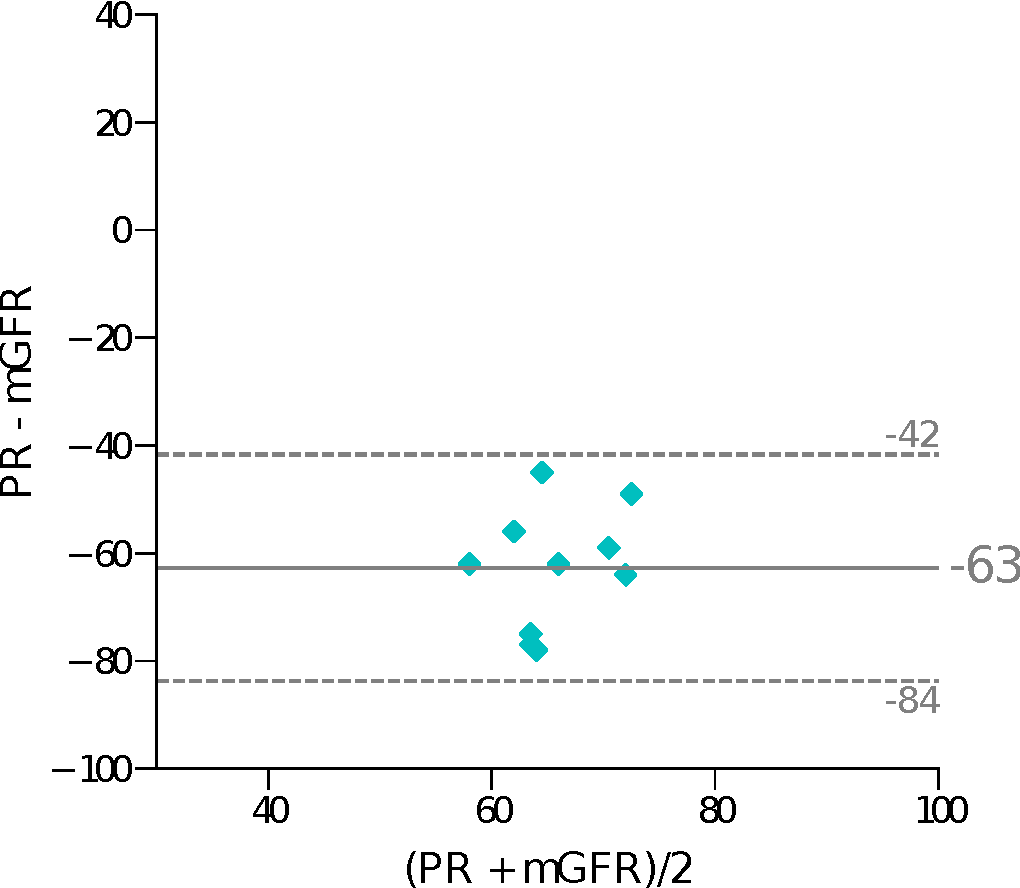
\includegraphics[width=0.42\linewidth]{baltman-pr}} \hfill \sidesubfloat[]{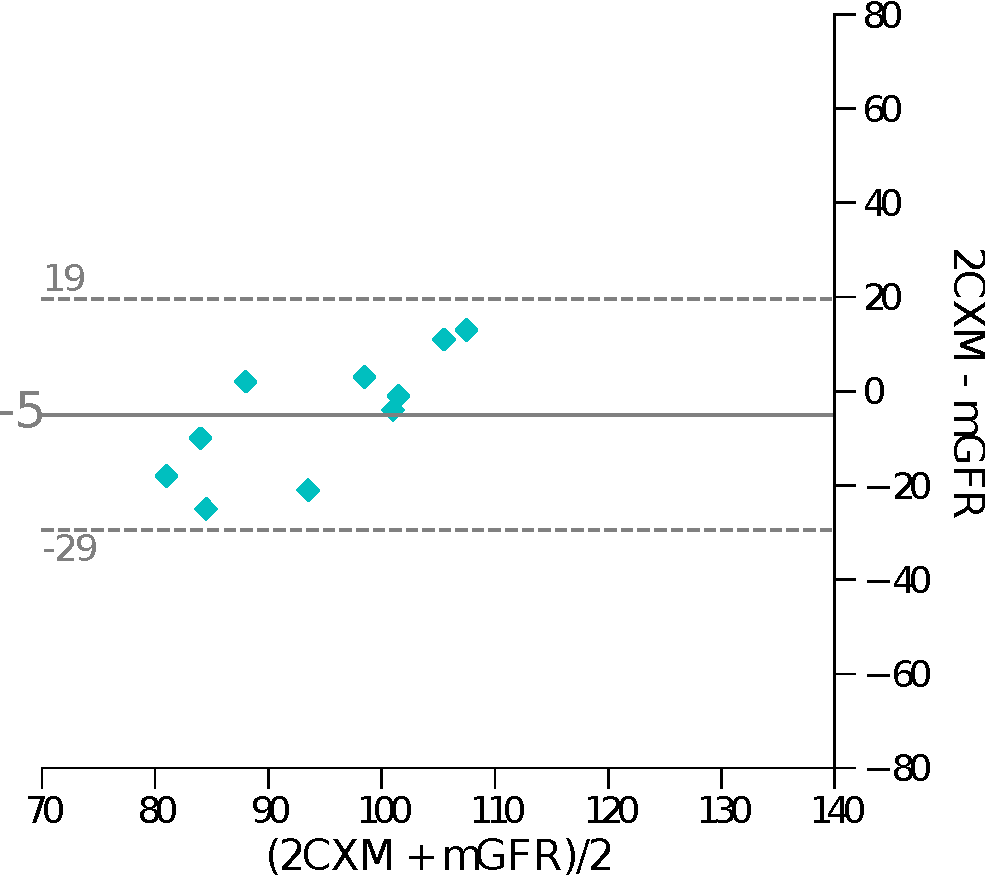
\includegraphics[width=0.42\linewidth]{baltman-2cxm}}
%\vspace{0.25cm}
\caption[Bland–Altman plots for different methods]{Bland–Altman plots for eGFR and different PK models with mGFR as a~reference. TK, ETK, PR, 2CXM are particular models. All measurements are given in mL/min/1.73\,m$^2$. Note that for PR model the scale is different because of large shifts} 
\label{fig:baltman}
\end{figure}

Table \ref{tab:results2} compares the performance of PK models and SCr blood test (eGFR). For every of the method the average absolute error, defined as the absolute difference between mGFR and GFR obtained by the particular method was calculated.
The goodness of fit of the model was evaluated with \textit{root mean squared error} (RMSE). 
Additionally, for every of the GFR measurement method, the P30 value was calculated, which is the percent of the measurements lying within $\pm\,30\%$ of the true value (iohexol-GFR).

\begin{table}[H]
\centering
\caption[Comparison of different GFR estimation methods]{Average absolute error, root mean square error, $P30$, bias and limits of agreement for different GFR estimation methods} 
\label{tab:results2}
\begin{threeparttable}
\rowcolors{2}{}{middleblue!30}
\renewcommand{\arraystretch}{1.5}
\begin{tabular}{l R{2.5cm} R{2.5cm}  R{2cm} R{2cm} R{2cm}}
	\toprule

	\textbf{Method} & \textbf{Average absolute error}  & \textbf{RMSE}    & \textbf{P30}   & \textbf{bias} & \textbf{LoA} \\ \toprule
				eGFR  & 		15\,$\pm$\,7     		 	 & ---  				&	100\,\%      &  13  & -6--33 \\
				 TK   & 		23\,$\pm$\,24    			 & 6.91\,$\pm$\,0.89		        & 	70\,\%       & 23   &  -23--69 \\
				ETK   & 		16\,$\pm$\,11     			 & 5.64\,$\pm$\,0.63			        &	80\,\%       &0    & -38--38\\
				 PR   & 		63\,$\pm$\,11     			 & 9.26\,$\pm$\,1.27				        &	  0\,\%      & -63  & -84--\,-42\\
			    2CXM  & 		11\,$\pm$\,9     		     & 5.15\,$\pm$\,0.60				        &	  100\,\%      &  -5  & -29-19\\
				

  	\bottomrule

\end{tabular}
\begin{tablenotes}%
\footnotesize{}%
\item Average absolute error, RMSE, bias and LoA are given in mL/min$^{-1}$/1.73\,m$^2$
    \end{tablenotes}
	\end{threeparttable}
\end{table}


Additionally, the correlations of the GFR values obtained by PK modelling and SCr test from mGFR were evaluated with the Pearson correlation coefficient, $r$ and the p-value, $p$ for this test was determined. Obtained values as well as the best linear fits are presented in Figure~\ref{fig:regression}.  
\newpage

\begin{figure}[H]
%\captionsetup[subfigure]{labelformat=empty,textformat=simple}
	\centering
	\sidesubfloat[]{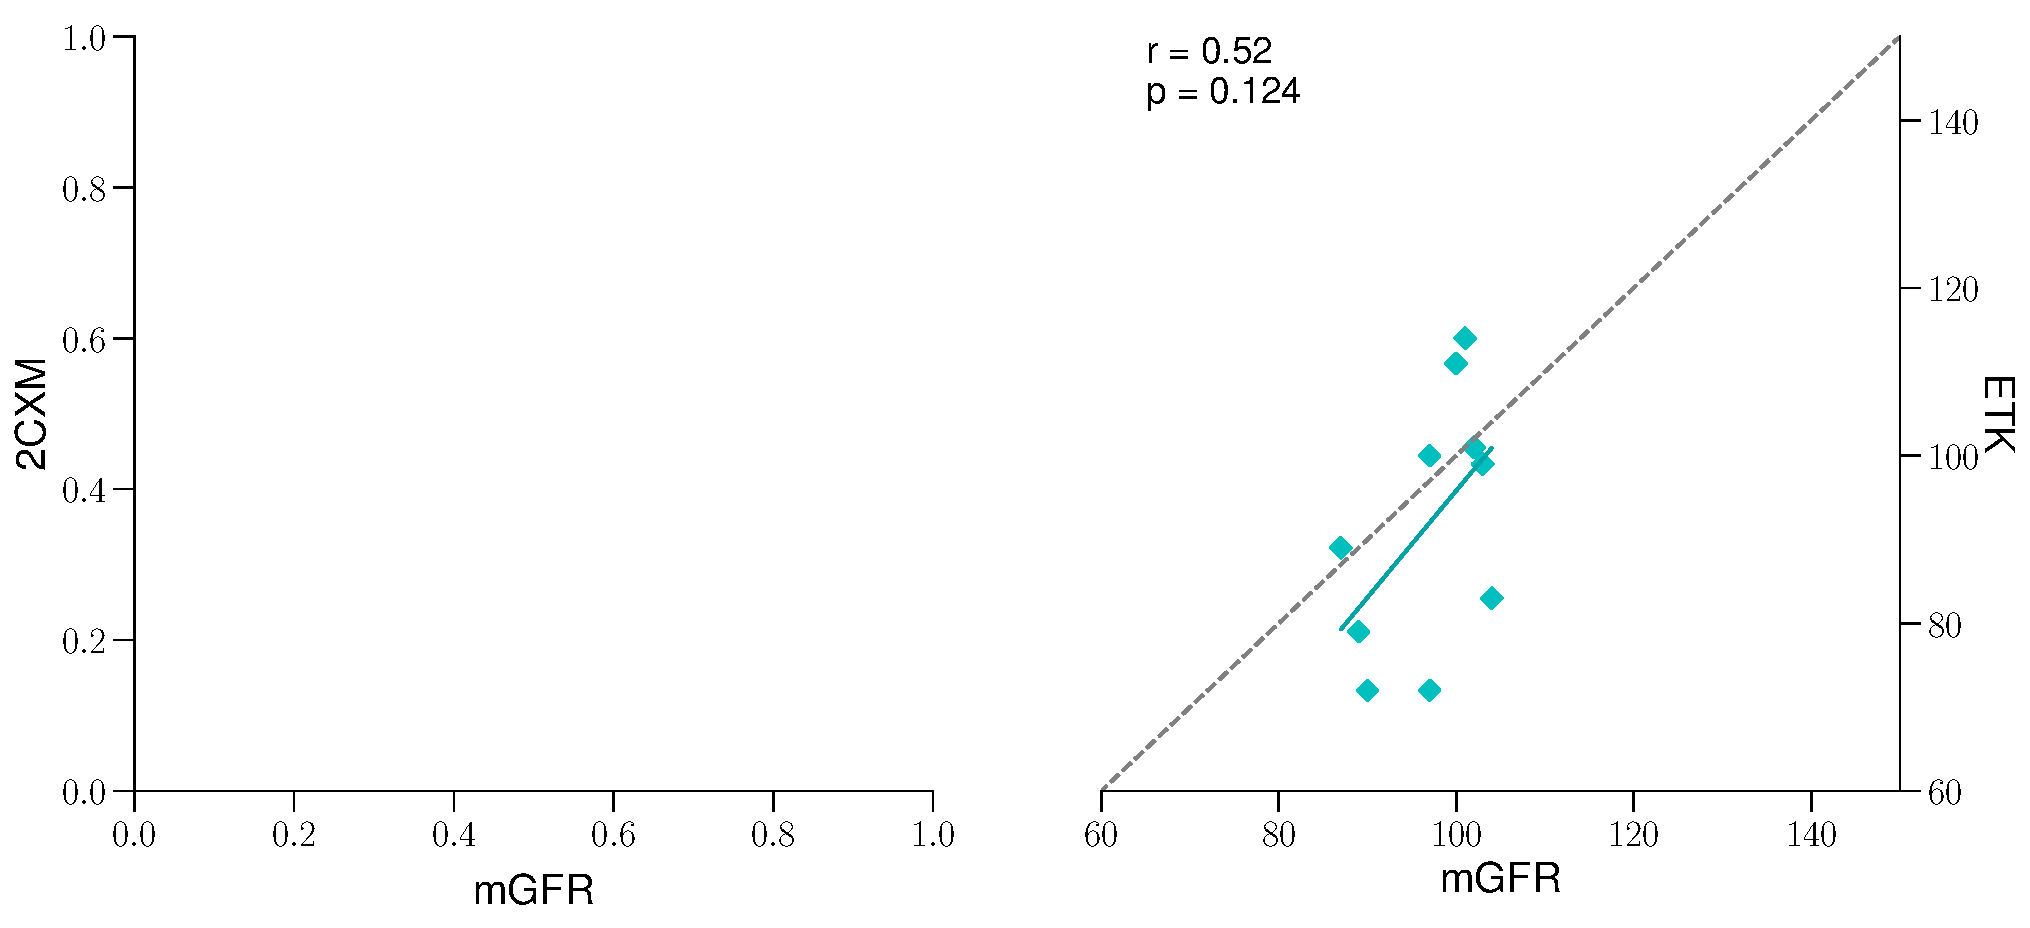
\includegraphics[width=0.42\linewidth]{reg-egfr}} \\ \vspace{10pt}  
 	\sidesubfloat[]{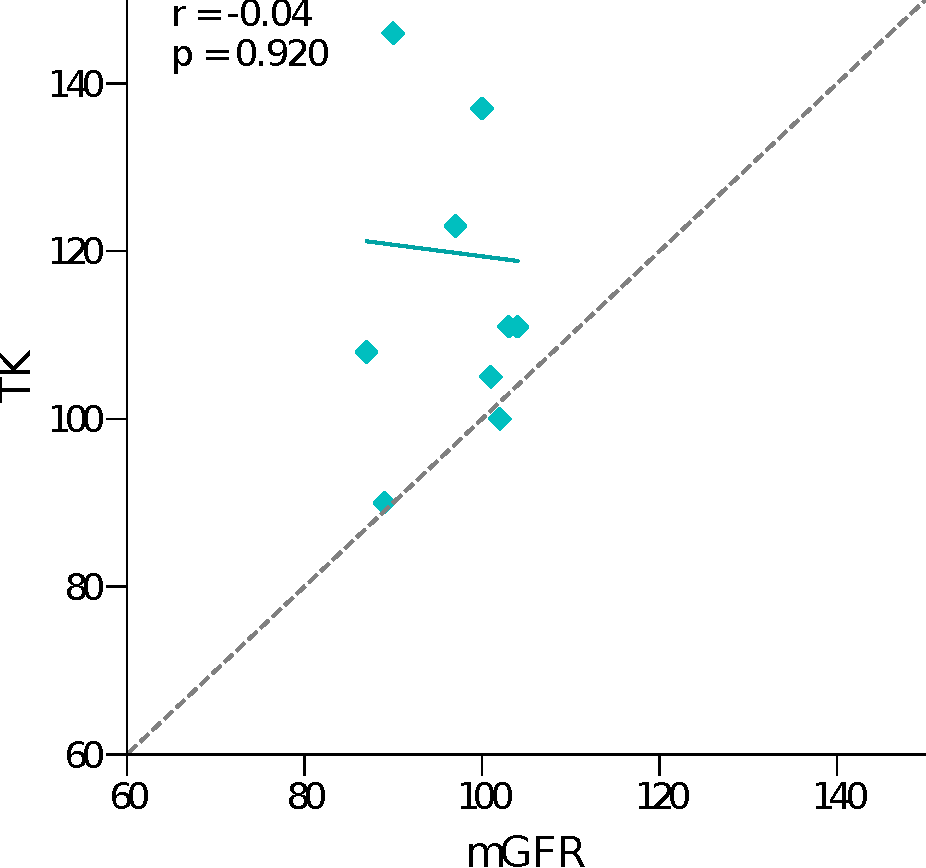
\includegraphics[width=0.42\linewidth]{reg-tk}} \hfill \sidesubfloat[]{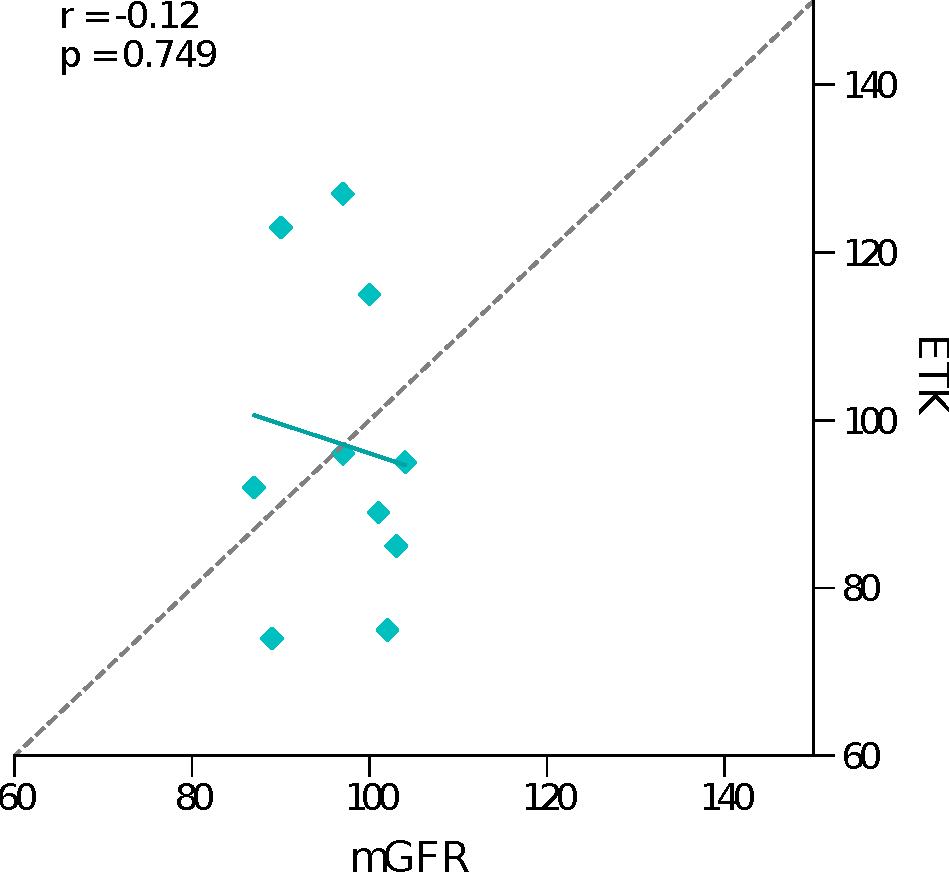
\includegraphics[width=0.42\linewidth]{reg-etk}} \\ \vspace{10pt}   
	\sidesubfloat[]{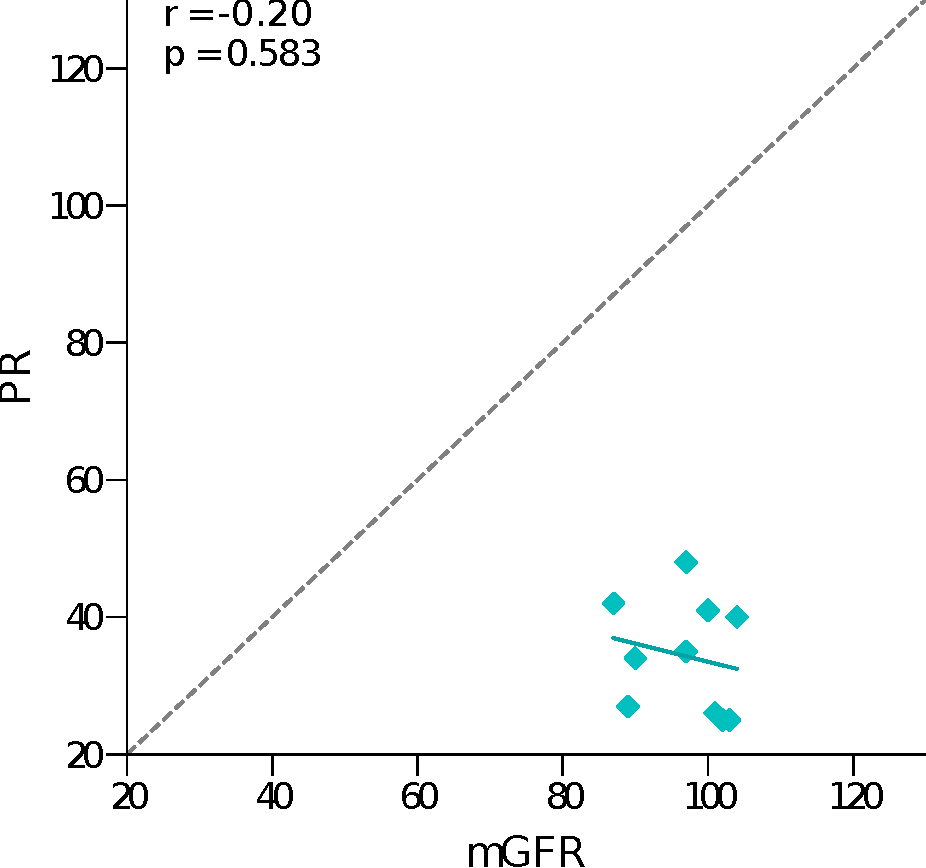
\includegraphics[width=0.42\linewidth]{reg-pr}} \hfill \sidesubfloat[]{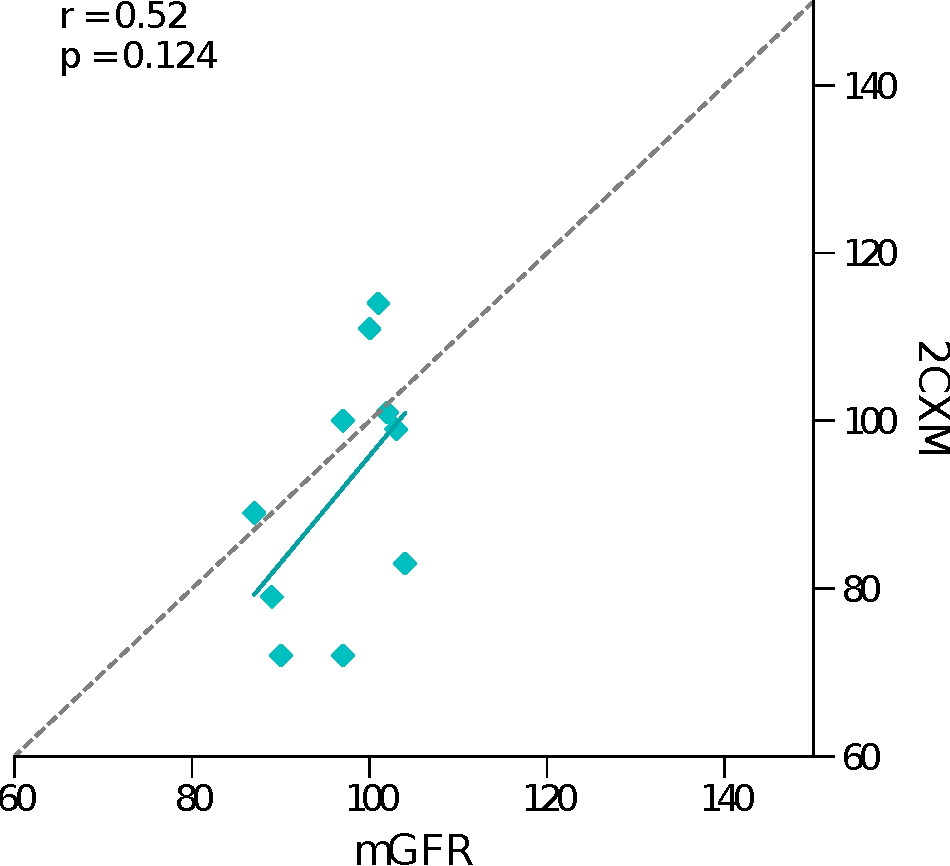
\includegraphics[width=0.42\linewidth]{reg-2cxm}}
	%\vspace{0.25cm}

\caption[Relation between mGFR and different estimation method]{Relation between mGFR and (a) eGFR (b-e) different PK models. The dashed grey line indicates equality, whereas robust blue one the best linear fit. All measurements are given in mL/min/1.73\,m$^2$; $r$: Pearson correlation coefficient, $p$~:~p-value } 
\label{fig:regression}
\end{figure}
  
  

